\section{The Sacred Center}

\begin{quotex}
You are the clearest and most magnificent denotation of God, for you have it in you to glorify Him through yourself. ... You are His greatest name.
\flright{\textsc{Ibn Arabi}}
\end{quotex}



\begin{wrapfigure}{rt}{.3\textwidth}
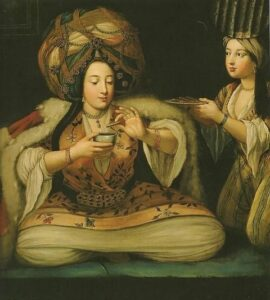
\includegraphics[width=.3\textwidth]{EnjoyingCoffee-270x300.jpg}
\end{wrapfigure}

\textbf{Naida}, the Mastermind behind \textit{Orphic Inscendence}\footnote{\url{https://www.orphicinscendence.com/post/the-sacred-center}}, leads us on a journey to the center. First, in the ancient city the place of worship was at the city center. Pagans kept the hearth burning at the center.

There are other examples, including a novel understanding of Prometheus. Even the simple act of sharing a cup of coffee has significance, as long as the experience points to the center.

She tells us:

\begin{quotex}
When a human being comes in knowledge of the Self beyond every other self, that human being sets his or her own flame ablaze. It begins to burn and lights up everything around. It gives a Center and the Center gives the ground and basis for every experience.
\end{quotex}


Once the significance of the fire brought to us by Prometheus has been grasped, one can not longer roam aimlessly around the outskirts, the outer boundaries, like an untamed lion peeing on the bushes to mark his territory. A dim memory of our true source drives us back to the center:

\begin{quotex}
When a fire of desire to know has been lit, a human being begins to move towards the Self, that is, towards the Unity and the Paradise. Reaching it, a human being becomes once again what the human being was before forgetting.
\end{quotex}


For the complete text, please visit \emph{Remembering the Sacred Center}\footnote{\url{https://www.orphicinscendence.com/post/the-sacred-center}} at Orphic Inscendence.


\flrightit{Posted on 2021-02-26 by Cologero}

\begin{center}* * *\end{center}

\begin{footnotesize}
\begin{sffamily}
\texttt{Rusalka on 2021-02-28 at 04:11 said:}

Thank you!


\hfill

\end{sffamily}
\end{footnotesize}

